\section{Warmup: A direct proof for preorder sequences}
\label{sec:warmup}


In this section we show that the cost of \greedy on an arbitrary preorder access sequence is linear. In other words, we give a direct proof of Corollary~\ref{cor:trav2}. We assume the preprocessing discussed in \S\,\ref{sec:prelim-short}, or equivalently, in geometric view we assume that \greedy runs with no initial tree\footnote{Curiously, in the case of \greedy and preorder sequences this has the same effect as if the initial tree would be exactly the tree that generated the input sequence.}, i.e.\ initially all stairs are empty.
%%This result can be seen as the geometric analogue of the \emph{traversal conjecture} for splay trees. 
%%The proof of the general preorder access sequences appears in the next section. 
The proof is intended as a warmup, to develop some intuition about the geometric model and to familiarize with the concepts of \emph{wings} and \emph{hidden elements} used in the subsequent proofs. We remark that an alternative proof of the same result (up to the same constants) can be obtained using forbidden submatrix arguments. %Later, wing will be defined slightly differently, but the definitions will capture almost idential ideas. 


\paragraph{Preorder sequences.} The class ${\sf PreOrd}_n$ of preorder sequences of length $n$ can be defined recursively as follows. A permutation sequence $X = (x_1, \dots, x_n)$ belongs to ${\sf PreOrd}_n$ if (i)$|X| = n = 1$ or (ii) there is a number $n' < n$, such that  
\begin{itemize} 
 \item $L(X) = (x_2,\ldots, x_{n'}) \in \sf{PreOrd}_{n'-1}$, 
 \item $R(X) = (x_{n'+1},\ldots, x_n) \in \sf{PreOrd}_{n - n'}$,
% \item $ \max_{x_t \in L} x_t  < x_1 < \min_{x_t \in R} x_t$.
 \item $ \max{\{L(X)\}}  < x_1 < \min{\{R(X)\}}$.
\end{itemize}

We remark again the well-known fact that preorder sequences are exactly the $(2,3,1)$-free permutations, and the easily verifiable fact that preorder sequences are 2-decomposable (see Figure~\ref{fig:preorder-seq} for an illustration).  
\begin{figure}[h]
\centering
%\includegraphics[scale=0.6, trim= 0cm 2in 0in 0.2in]{preorder-sequence.pdf}
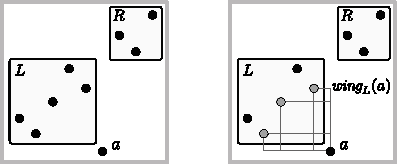
\includegraphics[scale=1.4]{fig_preorder.pdf}
\caption{Preorder sequence with sets $L$ and $R$, with $\textit{wing}_L(a)$  highlighted. Observe that point $a$ together with $L$ can form a single block.}
\label{fig:preorder-seq}
\end{figure}

We prove the following theorem.



\begin{theorem}~\label{thm:greedy-traversal}
Let $X \in {\sf PreOrd}_n$. Then $\mbox{{\sc Greedy}}(X) \leq 4n$.
\end{theorem}

%\lk{work-in-progress}
%%For element $a$, let $\tset_{a}$ be the subtree rooted at $a$.  


%and let $\wing_{L}(a)$ and $\wing_{R}(a)$ be defined as follows.

%\subsection{The Wings, Hidden Elements, and Forbidden Patterns}
\subsection{Wings and hidden elements}
\label{sec:wing-hidden}

%%The notion of {\em wings} will be crucial for the analysis in Section~\ref{sec:decomposition}.  
  
Let $X \in {\sf PreOrd_n}$. For an arbitrary element $a \in X$, let $t_a$ denote its access time. Let $L_a$ denote the maximal contiguous subsequence of $X$ immediately after $a$, that consists of elements smaller than $a$. Let $r_a \in X$ be the smallest element that is larger than $a$ and precedes $a$ in $X$. By convention, $r_a$ is $\infty$ if there are no elements larger than $a$ that precede $a$ in $X$. Let $R_a$ denote the maximal contiguous subsequence after $L_a$ of elements larger than $a$ and smaller than $r_a$.


%%Let $R_a$ denote the maximal contigous subsequence of $X$ immediately after $L_a$, that consists of elements greater than $a$. 

Let $\tset_a$ be the concatenation of $L_a$ and $R_a$. Let $\textit{lca}(b,c)$ denote the last element $a$, such that $b,c \in \tset_a$.

%\laszlo{should we mention that these correspond to subtrees, or try to do without trees?} 
We define $wing_L(a)$ to contain all elements $b \in L_a$ such that the rectangle with corners $(b, t_b)$, $(a,t_a)$ contains no other access point. Symmetrically, we define $wing_R(a)$ to contain all elements $b \in R_a$ such that the rectangle with corners $(b, t_b)$, $(a,t_a)$ contains no other access point (Figure~\ref{fig:preorder-seq}).

\begin{lemma} 
The sets $\set{ wing_L(a)}_{a \in [n]}$ are disjoint.  
Similarly, the sets $\set{wing_R(a)}_{a \in [n]}$ are disjoint.  
\end{lemma} 
\begin{proof}
Assume for contradiction that there are two elements $a, a' \in [n]$ such that $wing_L(a) \cap wing_L(a') \neq \emptyset$. Assume w.l.o.g.\ that $a<a'$. By definition, $wing_L(a)$ only contains elements in $L_a$, so there must be an element $b \in L_a \cap L_{a'}$, such that $b<a<a'$ and $t_b>t_a$ and $t_b>t_a'$. There are two possibilities: either $t_a > t_a'$, contradicting the fact that the rectangle with corners $(a',t_a')$, $(b,t_b)$ is empty, or $t_a < t_a'$, in which case the subsequence $(a, a', b)$ is order-isomorphic to $(2,3,1)$, contradicting the fact that $X$ is a preorder sequence.
%%This is impossible: In order for $(b,t_b)$ to have empty rectangle with both $(a,t_a)$ and $(a',t_{a'})$, the points $(a,t_a)$ and $(a', t_{a'})$ cannot dominate each other. Assume that $(a,t_a)$ is located bottom-left of $(a',t_{a'})$. Since $b \in L_a \cap L_{a'}$, the point $(b,t_b)$ is located above $t_{a'}$ and left of $a$. This creates a forbidden pattern $\rho$ in $X$, a contradiction.  
%But then both $a$ and $a'$ cannot have $b$ in their subtrees.   
\end{proof} 
The reader might find it instructive to see the corresponding situation in tree-view. Figure~\ref{leftwingpart} shows a proof by picture in the tree corresponding to the preorder sequence $X$.  


\begin{figure}[h]
\centering
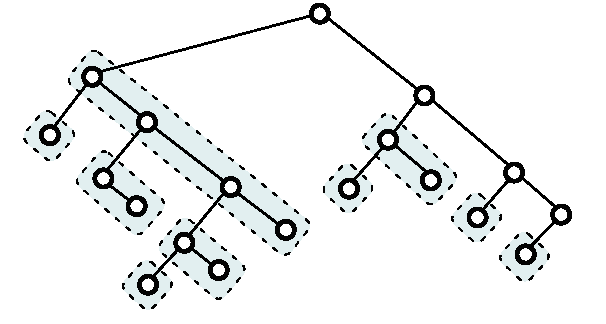
\includegraphics[width=3.5in]{LeftwingPartition_fig.pdf}
\caption{BST corresponding to a preorder sequence. Left wings of elements indicated as shaded rectangles.}
\label{leftwingpart}
\end{figure}

\begin{corollary} 
$\sum_a (|wing_L(a)| + |wing_R(a)|) \leq 2n$. 
\end{corollary}  


%%The following observations refer to the execution of {\sc Greedy} on the preorder sequence $X$. 

Next we restate and prove Lemma~\ref{prop:hidden} about hidden elements. Recall that $\tau(x,t-1)$ denotes the last time strictly before $t$ when $x$ is touched. 

\begin{definition}[Definition~\ref{def:hidden}]
	For any algorithm $\cA$, an element $x$ is \emph{hidden in} range $[w,y]$ after $t$ if,
	given that there is no access point $a \in [w,y]\times(t,t']$ for any $t'>t$, then
	 $x$ will not be touched by $\cA$ in time $(t,t']$.
\end{definition}

\begin{lemma} [Lemma~\ref{prop:hidden}]
Let $x$ be some element.
\begin{compactenum}[(i)]
\item If there is an element $w<x$ where $\tau(w,t)\ge\tau(x,t)$, then
$x$ is hidden in $(w,n]$ and $(w,x]$ after $t$ for \greedy and \greedyright respectively.
\item If there is an element $y>x$ where $\tau(y,t)\ge\tau(x,t)$, then
$x$ is hidden in $[1,y)$ and $[x,y)$ after $t$ for \greedy and \greedyleft respectively.
\item If there are elements $w,y$ where $w<x<y$, and $\tau(w,t),\tau(y,t)\ge\tau(x,t)$, then
$x$ is hidden in $(w,y)$ after $t$ for \greedy.
\end{compactenum}
\end{lemma}
\begin{proof}
\begin{compactenum}[(i)]
\item Consider any $t'>t$. For the case of \greedy, assume that there is no access point in $(w,n] \times (t,t']$. Suppose $x$ is touched in the time interval $(t,t']$, and let $(p,t_p)$ be the first access point in this time interval that causes the touching of $x$. Then $p \in [1,w]$, and $t_p \in (t,t']$. As $x$ is not touched in the time interval $(t,t_p)$ by the choice of $p$, we have that $\tau(x,t_p-1) = \tau(x,t)$. If $\tau(w,t)\ge\tau(x,t)$, then the rectangle with corners $(p,t_p)$, and $(x,\tau(x,t_p-1))$ contains the point $(w,\tau(w,t))$, and thus it is satisfied before accessing $p$. Therefore, the accessing of $p$ via \greedy does not touch $x$, a contradiction. It follows that $x$ is hidden in $(w,n]$ for \greedy after $t$.

For the case of \greedyright, assume that there is no access point in $(w,x] \times (t,t']$. Suppose $x$ is touched in the time interval $(t,t']$, and let $(p,t_p)$ be the first access point in this time interval that causes the touching of $x$. Then $p \in [1,w]$, and $t_p \in (t,t']$. (The case $p \in (x,n]$ is not possible for \greedyright, since $p<x$ must hold.) The remainder of the argument is the same as for \greedy.

\item The argument is symmetric to (i). 
\item Consider any $t'>t$. Assume that there is no access point in $(w,y) \times (t,t']$. Suppose $x$ is touched in the time interval $(t,t']$, and let $(p,t_p)$ be the first access point in this time interval that causes the touching of $x$. There are two cases. If $p \in [1,w]$, we use the argument of (i). If $p \in [y,n]$, we use the argument of (ii).
\end{compactenum}
\end{proof}

\iffalse
Let $I = [t',t'']$ be a time interval and let $x$ be an element. We say that $x$ is \emph{$[t',t'']$-hidden} if there is a range $R = [v,z] \subseteq [n] $ such that: 
\begin{compactenum}[--]
%%\item $x \in R$ and 
\item no element in $R$ is accessed in $I$. 
\item if there is an access to an element greater than $x$ in $I$, then there is a $y \in (x,z]$ with $\tau(y,t') \ge \tau(x,t')$. 
\item if there is an access to an element smaller than $x$ in $I$, then there is a $w \in [v,x)$ with $\tau(w,t') \ge \tau(x,t')$. 
\end{compactenum}
We also say that \emph{$x$ is $I$-hidden via range $R$} if $R$ satisfies the above.
See Figure~\ref{fig: hidden}. 


\begin{lemma} 
\label{lem: hidden lemma}
Let $I$ be a time interval and $x$ be an element that is $I$-hidden. 
Then $x$ is not touched in $I$. \end{lemma}
\begin{proof} Let $I = [t',t'']$ and $R = [v,z]$ and $y$ and $w$ as in the definition of $I$-hidden. 


Assume for the sake of contradiction that $x$ is touched during $I$. Let $t \in I$ be the first time, when $x$ is touched during $I$. Then $\tau(t,x) = \tau(t',x)$. We may assume that the access at time $t$ is to an element greater than $z$. By assumption, there is a $y \in (x,z]$ with $\tau(y,t') \ge \tau(x,t')$. Since $\tau(y,t) \ge \tau(y,t')$, 
the rectangle with corners $(x,\tau(x,t)),(z,t)$ contains $(y,\tau(y,t))$ and hence $x$ is not touched at time $t$.
\end{proof}
\fi

\subsection{Bounding the cost of \greedy}  

\begin{lemma}
For any element $c\in L_a \setminus \wing_{L}(a)$, $a$ is not touched when accessing $c$ using \greedy. Similarly for $c \in R_a \setminus wing_R(a)$.  
\end{lemma}
\begin{proof}
There must be an access point $b$, such that $c<b<a$ and $t_a<t_b<t_c$, for otherwise $c$ would be in $\wing_{L}(a)$. Since $\tau(b,t_b) \geq \tau(a,t_b)$, it follows that $a$ is hidden in $(b,n]$ after $t_b$. All accesses in the interval $(t_b, t_c]$ are in $[c,b)$. Hence, $a$ is not touched.
\end{proof}
\begin{corollary}\label{lem_pre1} Let $a$ be any element. 
\greedy touches $a$ when accessing elements in $\tset_a$ at most $|wing_L(a)| + |wing_R(a)|$ times.  
\end{corollary}

\begin{lemma}\label{lem_pre2} Let $a$ be any element. \greedy touches $a$ when accessing elements outside $\tset_a$ at most once. \end{lemma}
\begin{proof}
No element is touched before it is accessed. Since the elements in $\tset_a$ are accessed consecutively, we only need to consider accesses after all elements in $\tset_a$ have been accessed. All such accesses are to elements to the right of $\tset_a$. Let $c$ be the first element accessed after the last access to an element in $\tset_a$ and let $b = \mathit{lca}(a,c)$. Then $a \in L_b$, and $c$ is the first element in $R_b$. 

Since $\tset_c$ contains all elements in $(b,c]$, \greedy does not touch any element in $(b,c]$ before time $t_c$. Let $d$ be the element in $(a,b]$ with largest time $\tau(d,t_c-1)$. If there are several such $d$, let $d$ be the rightmost such element. Since no element in $(b,c]$ is accessed before time $t_c$, $d$ is also the rightmost element in $(a,c]$ with largest time $\tau(d,t_c-1)$. The rectangle with corners $(d,\tau(d,t_c-1))$ and $(c,t_c)$ contains no other point and hence $d$ is touched at time $t_c$. 

Clearly, $\tau(a,t_c) \le t_c = \tau(d,t_c)$. Thus $a$ is hidden in $[1,d)$ after time $t_c$ and hence $a$ is not touched after time $t_c$. 
\end{proof} 



Corollary~\ref{lem_pre1} and Lemma~\ref{lem_pre2} together imply that each element $a$ is only touched at most $|wing_L(a)| + |wing_R(a)| +1$ times, so the total cost is at most $\sum_{a \in [n]} (|wing_L(a)| + |wing_R(a)| +2) \leq 4n$.
This concludes the proof of Theorem~\ref{thm:greedy-traversal}.     
